\subsection{Content of an element of a free module}

Let A be a principal ideal domain, let L be a free A-module, and let x be an element of L. As f runs through the set \(L^{*}\) of linear forms on L, the elements \(f(x)\) form an ideal \(\mathfrak{c}_{\mathrm{L}}(x)\) of A, called the content of x in L. An element c of A is called a content of x in L if it generates the ideal \(\mathfrak{c}_{\mathrm{L}}(x)\) ; this amounts to saying that there exists a linear form f on L such that \(f(x)=c\) and that c divides \(g(x)\) for every linear form g on L. Let \((e_{i})_{i\in I}\) be a basis of L; put \(x=\sum a_{i}e_{i}, a_{i}\in A\) ; then the ideal \(\mathfrak{c}_{\mathrm{L}}(x)\) consists of sums \(\sum a_{i}b_{i}\) , as \((b_{i})\) runs through the set \(A^{I}\) ; it follows immediately that an element c of A is a content of x in L if and only if it is a gcd of the family \((a_{i})\) of coordinates of x.

We say that x is indivisible if \(\mathfrak{c}_{L}(x)=\mathbf{A}\) , that is if the coordinates of x with respect to a basis of L are setwise coprime.

Lemma 1. --- Let L be a free module over a principal ideal domain A and let x be an element of L. Then the following conditions are equivalent :

\begin{enumerate}
\def\labelenumi{(\roman{enumi})}
\item
  \(x\) is indivisible;
\item
  there exists a linear form \(f\) on \(L\) such that \(f(x) = 1\) ;
\item
  \(x\) is nonzero and the submodule \(\mathbf{A}x\) is a direct factor of \(\mathbf{L}\) ;
\item
  \(x\) is an element of some basis of \(\mathbf{L}\) .
\item
  \(\Rightarrow\) (ii): this follows from the definition.
\item
  \(\Rightarrow\) (iii): let \(f\) be a linear form on \(\mathbf{L}\) such that \(f(x) = 1\) ; then \(x \neq 0\) and the map \(y \mapsto f(y)x\) is a projector of \(\mathbf{L}\) , with image \(\mathbf{A}x\) .
\item
  \(\Rightarrow\) (iv): let \(L'\) be a complement of \(Ax\) in \(L\) , and let \(B'\) be a basis of \(L'\) (VII, p.~15, Cor. 2); then \(B' \cup \{x\}\) is a basis of \(L\) .
\item
  \(\Rightarrow\) (i): trivial.
\end{enumerate}

Remarks. --- 1) If \(x\) is a nonzero element of \(L\) and \(c\) a content of \(x\) , then there exists a unique element \(y\) of \(L\) such that \(x = cy\) ; denote this element \(x / c\) ; then \(x / c\) is an indivisible element of \(L\) .

\begin{enumerate}
\def\labelenumi{\arabic{enumi})}
\setcounter{enumi}{1}
\tightlist
\item
  The content \(\mathfrak{c}_{\mathrm{L}}(x)\) is the annihilator of the torsion module of \(\mathrm{L} / \mathrm{A}x\) .
\end{enumerate}

Let L be a free module over a principal ideal domain A and let M be a submodule of L; by VII, p.~4, Lemma 1, the family \(\mathfrak{c}_{\mathrm{L}}(x)\) , \(x \in M\) , has a maximal element; if \(M \neq \{0\}\) then such a maximal element is nonzero.

PROPOSITION 3. --- Let L be a free module over a principal ideal domain A and let M be a nonzero submodule of L. Let x be an element of M such that \(\mathfrak{c}_{\mathrm{L}}(x)\) is maximal among the contents of elements of M, let c be a content of x in L, and let f be a linear form on L such that \(f(x) = c\) .

\begin{enumerate}
\def\labelenumi{\alph{enumi})}
\item
  L is the direct sum of A(x/c) and the kernel K of f.
\item
  \(\mathbf{M}\) is the direct sum of \(\mathbf{A}\mathbf{x}\) and \(\mathbf{K} \cap \mathbf{M}\) .
\item
  \(g(M) \subset Ac\) for every linear form \(g\) on \(L\) .
\end{enumerate}

Put \(y = x / c\) ; clearly \(\mathbf{A}y \cap \mathbf{K} = \{0\}\) , since \(f(y) = 1\) . Furthermore, for each \(u \in L\) we have

\[
u = f (u) y + (u - f (u) y),
\]

with \(f(u) y \in \mathbf{A}y\) and \(u - f(u)y \in \mathbf{K}\) ; this proves \(a\) ). Now note that for \(u \in \mathbf{M}\) we have \(f(u) \in \mathbf{A}c\) : indeed, let \(u \in \mathbf{M}\) , and let \(d\) be a gcd of \(f(u)\) and \(c\) ; then there exist \(\lambda, \mu \in \mathbf{A}\) such that \(d = \lambda f(u) + \mu c = f(\lambda u + \mu x)\) ; hence the content of the element \(\lambda u + \mu x\) of \(\mathbf{M}\) divides \(d\) ; by the maximality of \(c\) , this implies that \(d\) is an associate of \(c\) , so \(f(u) \in \mathbf{A}c\) . Hence for all \(u\) in \(\mathbf{M}\) , we can write

\[
u = (f (u) / c) x + (u - (f (u) / c) x) \in \mathrm{A} x + (\mathrm{K} \cap \mathrm{M}),
\]

which shows \(b\) ). Finally, let \(g\) be a linear form on \(L\) ; by \(a\) ) there exists a scalar \(\alpha \in A\) and a linear form \(h\) on \(K\) such that \(g(u) = \alpha f(u) + h(u - f(u)y)\) ; thus by b) we have \(g(\mathbf{M}) \subset \mathbf{A}c + h(\mathbf{K} \cap \mathbf{M})\) . To prove c), it is therefore sufficient to prove that \(h(\mathbf{K} \cap \mathbf{M}) \subset \mathbf{A}c\) for every linear form h on K, or equivalently for every linear form h on L such that \(h(x) = 0\) ; now, if \(u \in K \cap M\) and d is a gcd of \(h(u)\) and c, then there exist \(\lambda\) , \(\mu \in A\) with \(d = \lambda h(u) + \mu c\) ; then \((f + h)(\lambda u + \mu x) = d\) , which implies as above that \(h(u) \in Ac\) , and c) follows.

\subsection{Invariant factors of a submodule}

THEOREM 1. --- Let L be a free module over a principal ideal domain A, and let M be a submodule of L of finite rank n.~Then there exist a basis B of L, n elements \(e_{i}\) of B, and n nonzero elements \(\alpha_{i}\) of A ( \(1 \leqslant i \leqslant n\) ) such that :

\begin{enumerate}
\def\labelenumi{\alph{enumi})}
\item
  the \(\alpha_{i}e_{i}\) form a basis of \(\mathbf{M}\) ;
\item
  \(\alpha_{i}\) divides \(\alpha_{i + 1}\) for \(1\leqslant i\leqslant n - 1\)
\end{enumerate}

Moreover the module M' generated by the \((e_{i})\) and the principal ideals \(A\alpha_{i}\) are uniquely determined by the above conditions; the module M'/M is the torsion submodule of L/M, and is isomorphic to the direct sum of the A-modules A/A \(\alpha_{i}\) ; finally L/M is the direct sum of M'/M and a free module isomorphic to L/M'.

\begin{enumerate}
\def\labelenumi{\arabic{enumi})}
\tightlist
\item
  Existence of the \(e_i\) and the \(\alpha_i\) .
\end{enumerate}

If \(M = \{0\}\) then the theorem is trivial. If \(M \neq \{0\}\) then it follows from Prop. 3 that there exist an element \(e_{1}\) of L, a nonzero element \(\alpha_{1}\) of A, and a submodule \(L_{1}\) of L, such that L is the direct sum of \(Ae_{1}\) and \(L_{1}\) , such that M is the direct sum of \(A\alpha_{1}e_{1}\) and the submodule \(M_{1} = M \cap L_{1}\) of L, and such that \(g(M) \subset A\alpha_{1}\) for every linear form g on L.

Now we can proceed by induction on the rank \(n\) of \(M\) . Since \(L_1\) is a free module (VII, p.~15, Cor. 2) and \(M_1\) has rank \(n - 1\) , there exist a basis \(B_1\) of \(L_1\) , \((n - 1)\) elements \(e_2, \ldots, e_n\) of \(B_1\) , and nonzero elements \(\alpha_2, \ldots, \alpha_n\) of \(A\) such that \((\alpha_2e_2, \ldots, \alpha_ne_n)\) is a basis of \(M_1\) , and \(\alpha_i\) divides \(\alpha_{i+1}\) for \(2 \leqslant i \leqslant n - 1\) . If \(L'\) is the submodule of \(L_1\) generated by the elements of \(B_1\) distinct from \(e_2, \ldots, e_n\) , then \(L\) is the direct sum of \(L'\) and the module \(M'\) generated by \(e_1, \ldots, e_n\) ; now \((e_1, \ldots, e_n)\) is a basis for \(M'\) , and \((\alpha_1e_1, \ldots, \alpha_ne_n)\) is a basis for \(M\) . It now remains only to show that \(\alpha_1\) divides \(\alpha_2\) ; but \(A\alpha_2\) has the form \(g(M_1)\) , where \(g\) is the linear form on \(L\) defined by \(g(e_2) = 1\) , \(g(e_i) = 0\) for \(i \neq 2\) , and \(g(L') = \{0\}\) ; and we have seen above that \(g(M_1) \subset A\alpha_1\) .

2) Uniqueness properties.

Since the \(\alpha_{i}\) are nonzero, the module \(\mathbf{M}'\) is the set of \(x\in L\) such that \(\beta x\in M\) for some \(\beta \neq 0\) in A; in other words \(\mathbf{M}' / \mathbf{M}\) is the torsion submodule of L/M. This uniquely determines \(\mathbf{M}'\) .

It is clear that \(M^{\prime}/M\) is isomorphic to the direct sum of the n cyclic modules \(A/A\alpha_{i}\) (II, p.~204, formula (26)). Let r be the number of the ideals \(A\alpha_{i}\) which are distinct from A: so that the first n-r ideals \(A\alpha_{i}\) are equal to A, and the last r are distinct from A. Then \(M^{\prime}/M\) is also isomorphic to the direct sum of the modules \(A/A\alpha_{n}, \ldots, A/A\alpha_{n-r+1}\) , where \(A\alpha_{n} \subset A\alpha_{n-1} \subset \ldots \subset A\alpha_{n-r+1} \neq A\) .

Thus the conditions of the Cor. to Prop. 2 (VII, p.~16) are satisfied: the ideals \(\mathbf{A}\alpha_{i}\) ( \(1 \leqslant i \leqslant n\) ) are thus uniquely determined by the module \(\mathbf{M}'/\mathbf{M}\) .

Since L is the direct sum of \(M'\) and \(L'\) , it follows that L/M is the sum of \(M'/M\) and \((L'+M)/M\) , and this sum is direct since \((L'+M) \cap M' = M\) ; on the other hand \((L'+M)/M\) is isomorphic to \(L'/(M \cap L')\) (I, p.~41, Th. 4, c)), that is to \(L'\) , which shows that \((L'+M)/M\) is a free module isomorphic to \(L/M'\) .

COROLLARY. --- A submodule M of finite rank in a free module L over a principal ideal domain A has a complement in L if and only if L/M is torsion free.

In the notation of Th. 1, if L/M is torsion free, then \(M = M'\) , and \(M'\) has a complement \(L'\) in L. Conversely if M has a complement \(L'\) in L, then L/M is isomorphic to \(L'\) , which is free (VII, p.~15, Cor. 2), and a fortiori torsion free.

Remark. --- It can happen that a submodule M of infinite rank in a free module L can be such that L/M is torsion free, but M has no complement in L (VII, p.~60, Ex. 6, b)).

DEFINITION 1. --- In the notation and hypotheses of Th. 1, the ideals \(A\alpha_{i}\) of A are called the invariant factors of the submodule M with respect to the module L.

In the case where A is either the ring Z of rational integers or the polynomial ring K{[}X{]} in one indeterminate over a field K, there is a canonical way of choosing a generator for each ideal of A: a positive integer in the case of Z, or a monic polynomial in the case of K{[}X{]} (VII, p.~5). In each of these cases, the canonical generator of the invariant factor \(A\alpha_{i}\) is also called an invariant factor of M with respect to L, by abuse of language.

\subsection{Structure of finitely generated modules}

THEOREM 2. --- Every finitely generated module E over a principal ideal domain A is isomorphic to a direct sum of a finite number m of cyclic modules \(A/a_{k}\) , where the \(a_{k}\) are ideals of A (some of which may be zero) such that \(a_{1} \subset a_{2} \subset \ldots \subset a_{m} \neq A\) , and which are uniquely determined by these conditions.

If E can be generated by q elements then it is isomorphic to a quotient module L/M, where \(L = A^{q}\) (II, p.~218). Since M has finite rank \(n \leqslant q\) (VII, p.~15, Prop. 1), the conditions of Th. 1 (VII, p.~18) are satisfied. Then in the notation of Th. 1 L/M is isomorphic to a direct sum of a complement \(L'\) of \(M'\) in L and the torsion module \(M'/M\) . The module \(L'\) is free of finite rank p = q - n, so isomorphic to \(A^{p}\) . If r is the smallest index such that \(A\alpha_{r} \neq A\) , then \(M'/M\) is isomorphic to the direct sum of modules \(A/A\alpha_{i}\) for \(r \leqslant i \leqslant n\) . The stated conditions will then be satisfied if we take \(m = p + (n - r + 1)\) , \(\mathfrak{a}_{k} = (0)\) for \(1 \leqslant k \leqslant p\) , and \(\mathfrak{a}_{p+j} = A\alpha_{n-j+1}\) for \(1 \leqslant j \leqslant n - r + 1\) . Uniqueness follows from the Cor. of VII, p.~16.

\pandocbounded{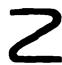
\includegraphics[keepaspectratio]{images/part003_91527dd3.jpg}}

COROLLARY 1. --- Every finitely generated module E over a principal ideal domain is the direct sum of the torsion submodule of E and a free module.

The torsion submodule of E has in general several distinct complements. For example, if \(E = \mathbf{Z} \times (\mathbf{Z}/(2))\) then the torsion submodule of E is \(\{0\} \times (\mathbf{Z}/(2))\) ; it has as a complement the submodule \(Z \times \{0\}\) , and also the submodule consisting of all elements \((n, \bar{n})\) , where n runs through Z and \(\bar{n}\) is the residue class of n mod 2.

COROLLARY 2. --- Every torsion free finitely generated module over a principal ideal domain is free of finite rank.

This follows immediately from Cor. 1.

\pandocbounded{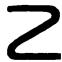
\includegraphics[keepaspectratio]{images/part003_b18cf4bc.jpg}}

The condition that the module be finitely generated is essential. For example the additive group of the field of fractions K of A is torsion free as an A-module; however it is not a free module if \(A \neq K\) , for on the one hand any two elements of K have a common divisor, and on the other hand K is not a cyclic A-module, for otherwise \(K = ab^{-1}A\) ( \(a, b \in A\) ), whence \(b^{-2} = acb^{-1}\) ( \(c \in A\) ), so \(b^{-1} = ac \in A\) , and K = A.

DEFINITION 2. --- In the notation and hypotheses of Th. 2, the ideals \(\mathfrak{a}_k\) are called the invariant factors of the module E.

As in Def. 1 (VII, p.~19), when A = Z or A = K{[}X{]}, the canonical generator of the ideal \(a_{k}\) (a positive integer or a monic polynomial) is also called, by abuse of language, an invariant factor of the finitely generated module E.

\pandocbounded{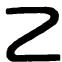
\includegraphics[keepaspectratio]{images/part003_8ba9a087.jpg}}

We must be careful not to confuse the invariant factors of a module E with those of a submodule M of a free module L with respect to the module L (Def. 1).

\subsection{Calculation of invariant factors}

PROPOSITION 4. --- Let A be a principal ideal domain, let L be a free A-module with finite basis \((u_{j})\) \((1 \leqslant j \leqslant k)\) , let M be a submodule of L, let \((x_{i})\) be a system of generators of M and let \(A\alpha_{i}\) \((1 \leqslant i \leqslant n)\) be the invariant factors of M with respect to L. Then for \(1 \leqslant m \leqslant n\) the product \(\delta_{m} = \alpha_{1} \ldots \alpha_{m}\) is a gcd of the m-th order minors of the matrix whose columns are the coordinate vectors of the \(x_{i}\) with respect to the basis \((u_{j})\) .

By Th. 1 it is clear that \(M \subset \alpha_{1}L\) ; hence the coordinates of any element of M are multiples of \(\alpha_{1}\) . On the other hand, there exists an element x of M for which \(\alpha_{1}\) is a content in L. Expressing x as a linear combination of the \(x_{t}\) , it follows that \(\alpha_{1}\) is an element of the ideal generated by the coordinates of the \(x_{t}\) . As these are all multiples of \(\alpha_{1}\) , it follows that \(\alpha_{1}\) is indeed their gcd, and our assertion is proved in the case m = 1.

For general \(m\) , consider the \(m\) -th exterior power \(\Lambda\) M of M (III, p.~507). In the notation of Th. 1 there exists a basis \((a_i)\) for M where \(a_i = \alpha_i e_i\) ( \(1 \leqslant i \leqslant n\) ); thus \(\Lambda\) M has a basis consisting of the elements \(a_{i_1} \wedge \ldots \wedge a_{i_m}\) , as \((i_1, \ldots, i_m)\) runs through the set of strictly increasing sequences of \(m\) elements of \((1, n)\) . Now the elements \(e_{i_1} \wedge \ldots \wedge e_{i_m}\) belong to a basis \(B_m\) of \(\bigwedge^m L\) . Hence the canonical map from \(\bigwedge^m M\) into \(\bigwedge^m L\) is an isomorphism from \(\bigwedge^m M\) onto the submodule of \(\bigwedge^m L\) having as a basis the elements \((\alpha_{i_1} \ldots \alpha_{i_m}) e_{i_1} \wedge \ldots \wedge e_{i_m}\) , and we identify this submodule with \(\bigwedge^m M\) . Since \(\alpha_j\) is a multiple of \(\alpha_k\) for \(j \geqslant k\) , the elements \(\alpha_{i_1} \ldots \alpha_{i_m}\) are all multiples of \(\delta_m = \alpha_1 \ldots \alpha_m\) , and one of them is equal to \(\delta_m\) ; thus \(\delta_m\) is a gcd of the coordinates with respect to \(B_m\) of the elements of a system of generators of \(\bigwedge^m M\) . The first part of the argument shows that then \(\delta_m\) is a gcd of the set of coordinates of any system of generators of \(\bigwedge^m M\) , with respect to any basis of \(\bigwedge^m L\) . Taking the basis for \(\bigwedge^m L\) induced from the basis \((u_j)\) of \(L\) , and the system of generators for \(\bigwedge^m M\) consisting of exterior products of the \((x_i)\) , the expression for the coordinates of these products in terms of determinants (III, p.~528, Prop. 9) gives the stated result.

\subsection{Linear mappings of free modules, and matrices over a principal ideal domain}

Let A be a principal ideal domain. Consider a linear mapping f from a free A-module L of rank m into a free A-module \(L'\) of rank n.~The preceding results allow us, by choosing suitable bases for L and \(L'\) , to put the matrix for f in a particularly simple form, called the canonical form of the matrix.

PROPOSITION 5. --- Let A be a principal ideal domain, and f a linear map of rank r from a free A-module L of rank m into a free A-module L' of rank n.~Then there exist bases \((e_{i})\) \((1 \leqslant i \leqslant m)\) of L and \((e_{j}')\) \((1 \leqslant j \leqslant n)\) of L' such that \(f(e_{i}) = \alpha_{i} e_{i}'\) for \(1 \leqslant i \leqslant r\) and \(f(e_{i}) = 0\) for i \textgreater{} r, where the \(\alpha_{i}\) are nonzero elements of A, each of which divides the next; the ideals \(A\alpha_{i}\) are the invariant factors of \(f(L)\) in \(L'\) , and are thus uniquely determined.

Let \(L_0 = f^{-1}(0)\) be the kernel of \(f\) ; the quotient \(L/L_0\) is isomorphic to the module \(f(L)\) , which is a submodule of \(L'\) and so free (VII, p.~15, Cor. 2); thus \(L_0\) has a complement \(L_1\) in \(L\) (II, p.~218, Prop. 21), and the restriction of \(f\) to \(L_1\) is an isomorphism from \(L_1\) onto \(f(L) = M'\) . If the ideals \(A\alpha_i\) ( \(1 \leqslant i \leqslant r\) ) are the invariant factors of \(M'\) in \(L'\) , then Th. 1 of VII, p.~18 shows that there exists a basis \((e_j')\) ( \(1 \leqslant j \leqslant n\) ) of \(L'\) such that \((\alpha_i e_i')\) ( \(1 \leqslant i \leqslant r\) ) is a basis of \(M'\) . Since the restriction of \(f\) to \(L_1\) is an isomorphism from \(L_1\) onto \(M'\) , there exists a basis \((e_i)\) ( \(1 \leqslant i \leqslant r\) ) of \(L_1\) such that \(f(e_i) = \alpha_i e_i'\) . This basis extends to a basis \((e_k)\) ( \(1 \leqslant k \leqslant m\) ) of \(L\) by taking \((e_s)\) ( \(r + 1 \leqslant s \leqslant m\) ) to be a basis of the kernel

\[
\mathbf {L} _ {0}
\]

COROLLARY 1. --- Let X be a matrix of rank r, with n rows and m columns, over a principal ideal domain A; then there exists a matrix \(X_{0}\) equivalent to X (II, p.~354) of the form

\[
\left( \begin{array}{c c c c c c c} \alpha_ {1} & 0 & \ldots & 0 & 0 & \ldots & 0 \\ 0 & \alpha_ {2} & \ldots & 0 & 0 & \ldots & 0 \\ 0 & 0 & \ldots & \alpha_ {r} & 0 & \ldots & 0 \\ 0 & 0 & \ldots & 0 & 0 & \ldots & 0 \\ 0 & 0 & \ldots & 0 & 0 & \ldots & 0 \end{array} \right)
\]

where the \(\alpha_{i}\) are nonzero elements of A, each of which divides the next. Under these conditions the \(\alpha_{i}\) are uniquely determined up to multiplication by invertible elements.

Given that two matrices X and \(X'\) are equivalent if there exist invertible square matrices P and Q, of orders n and m, over A, such that \(X' = PXQ\) , Cor. 1 is just Prop. 5 expressed in terms of matrices.

In the notation of Prop. 5 and Cor. 1, the (nonzero) ideals \(\mathbf{A}\alpha_{i}\) are called the invariant factors of the linear map \(f\) , or of the matrix \(X\) . It then follows immediately from Cor. 1 that:

COROLLARY 2. --- Two matrices X and \(X'\) with n rows and m columns over a principal ideal domain A are equivalent if and only if they have the same invariant factors.

Note that when A is a field we can take the \(\alpha_{i}\) to be equal to 1, and then we recover Prop. 13 of II, p.~360.

If X is the matrix of the linear mapping f with respect to an arbitrary basis of L and an arbitrary basis of \(L'\) , then the columns of X are the coordinate vectors, with respect to the basis of \(L'\) , of elements of \(L'\) which form a system of generators for \(f(\mathrm{L})\) . The following result is thus an immediate consequence of Prop. 4.

PROPOSITION 6. --- Let X be a matrix of rank r over a principal ideal domain A, and let \(A\alpha_{i}\) ( \(1 \leqslant i \leqslant r\) ) be its sequence of invariant factors. Then \(\alpha_{1}\) is a gcd of the elements of X; and the product \(\alpha_{1} \ldots \alpha_{q}\) is a gcd of the q-th order minors of X for \(q \leqslant r\) .

\subsection{Finitely generated abelian groups}

In the case \(\mathbf{A} = \mathbf{Z}\) , the results of section 4 can be expressed:

THEOREM 3. --- Every finitely generated abelian group G is a direct sum of its torsion subgroup F (subgroup of elements of finite order in G) and a free abelian group of finite rank p (isomorphic to \(Z^{p}\) ). The group F is a direct sum of a finite number of cyclic groups of orders \(n_{1}\) , \(n_{2}\) , \ldots, \(n_{q}\) , where the \(n_{i}\) are integers \textgreater1, each of which divides the previous one; moreover, the integers p, q and \(n_{i}\) ( \(1 \leq i \leq q\) ) are uniquely determined by G.

Remark. --- While the orders \(n_{1}, \ldots, n_{q}\) of the cyclic groups of which F is the direct sum are well defined by the divisibility condition of Th. 3, it is not the same for the groups themselves: for example, in the product G of \(\mathbf{Z}/(p)\) with itself (for p prime), the subgroups are precisely the \(F_{p}\) -vector subspaces, and G is the direct sum of two 1-dimensional subspaces in \(p(p+1)\) different ways.

COROLLARY 1. --- In a finite abelian group G, there exists an element whose order is the lcm of all the orders of elements of G; this order n is the first invariant factor of G.

COROLLARY 2. --- Any finite abelian group G whose order is not divisible by the square of any integer \textgreater1 is cyclic.

Let us keep to the notation of Th. 3. Then \(p = 0\) since \(G\) is finite, and \(q \leqslant 1\) , for otherwise the order of \(G\) would be divisible by \(n_q^2\) . Hence \(G\) is cyclic.

COROLLARY 3. --- Let L and M be two free Z-modules of rank n, let \((e_{i})\) be a basis for L and \((f_{i})\) a basis for M \((1 \leqslant i \leqslant n)\) , let u be a homomorphism from L into M, and let U be its matrix with respect to the bases \((e_{i})\) and \((f_{i})\) . Then Coker \(u = \mathrm{M}/u(\mathrm{L})\) is finite if and only if \(\det(U) \neq 0\) , and then \(\operatorname{Card}(\operatorname{Coker}(u)) = |\det(U)|\) .

By changing bases in L and M if necessary, we may assume that U has the form described in VII, p.~22, Cor. 1 to Prop. 5 (where the \(\alpha_{i}\) are in this case integers); the corollary then becomes obvious, since the order of a direct sum of Z-modules \(Z/\alpha_{i}Z\) ( \(1 \leqslant i \leqslant n\) ) is infinite if one of the \(\alpha_{i}\) is zero, and is equal to \(|\alpha_{1}\alpha_{2} \ldots \alpha_{n}|\) otherwise.

\subsection{Indecomposable modules. Elementary divisors}

DEFINITION 3. --- A left module M over a ring A is said to be decomposable if it is the direct sum of a family of proper nonzero submodules. Otherwise it is said to be indecomposable.

The zero module is thus decomposable, being the direct sum of the empty family of submodules.

Let \(\mathfrak{a}\) be a left ideal of the ring \(\mathbf{A}\) ; the submodules of \(\mathbf{A} / \mathfrak{a}\) are just the quotients \(\mathfrak{b} / \mathfrak{a}\) , where \(\mathfrak{b}\) is an ideal of \(\mathbf{A}\) containing \(\mathfrak{a}\) (I, p.~41, Th. 4); if \(\mathfrak{b}\) and \(\mathfrak{c}\) are two ideals of \(\mathbf{A}\) containing \(\mathfrak{a}\) , then the module \(\mathbf{A} / \mathfrak{a}\) is the direct sum of the submodules \(\mathfrak{b} / \mathfrak{a}\) and \(\mathfrak{c} / \mathfrak{a}\) if and only if \(\mathbf{A} = \mathfrak{b} + \mathfrak{c}\) and \(\mathfrak{b} \cap \mathfrak{c} = \mathfrak{a}\) . As a result:

Lemma 2. --- The module A/a is indecomposable if and only if a ≠ A and there is no pair (b, c) of ideals of A, distinct from A and a, such that A = b + c and b ∩ c = a.

PROPOSITION 7. --- Let A be a commutative ring, let p be a prime ideal of A (I, p.~117, Def. 3), and let q be an ideal of A contained in p.~Suppose that for every \(x \in p\) there exists an integer n \textgreater{} 0 such that \(x^{n} \in q\) . Then the A-module A/q is indecomposable.

Let \(\mathfrak{b}\) and \(\mathfrak{c}\) be two ideals of \(\mathbf{A}\) , such that \(\mathbf{A} = \mathfrak{b} + \mathfrak{c}\) and \(\mathfrak{b} \cap \mathfrak{c} = \mathfrak{q}\) . Then \(\mathfrak{bc} \subset \mathfrak{b} \cap \mathfrak{c} = \mathfrak{q} \subset \mathfrak{p}\) ; if \(x \notin \mathfrak{p}\) and \(x \in \mathfrak{c}\) , then \(xb \subset \mathfrak{p}\) , so \(\mathfrak{b} \subset \mathfrak{p}\) (I, p.~116, Prop. 4); hence either \(\mathfrak{b} \subset \mathfrak{p}\) or \(\mathfrak{c} \subset \mathfrak{p}\) . Suppose for example that \(\mathfrak{c} \subset \mathfrak{p}\) , so \(\mathfrak{b} + \mathfrak{p} = \mathbf{A}\) ; then there exist \(x \in \mathfrak{b}\) and \(y \in \mathfrak{p}\) such that \(1 = x + y\) ; let \(n \in \mathbf{N}\) be such that \(y^n \in \mathfrak{q}\) ; then \(1 = (x + y)^n\) , so \(1 \in x\mathbf{A} + y^n\mathbf{A} \subset \mathfrak{b} + \mathfrak{q} \subset \mathfrak{b}\) , so \(\mathfrak{b} = \mathbf{A}\) . Lemma 2 now shows that \(\mathbf{A}/\mathfrak{q}\) is indecomposable.

Now suppose that A is a principal ideal domain; by VII, p.~2, Prop. 2, the prime ideals of A are the ideals \((p)\) , where p is an irreducible element of A, and the ideal 0; by the previous proposition, the modules A and \(\mathbf{A}/(p^{n})\) , for p irreducible and n \textgreater{} 0, are indecomposable. Since every cyclic module is a direct sum of modules of this type (VII, p.~3, Prop. 4) and since every finitely generated A-module is a direct sum of cyclic modules (VII, p.~19, Th. 2), we deduce:

PROPOSITION 8. --- Let A be a principal ideal domain and let M be a finitely generated A-module.

\begin{enumerate}
\def\labelenumi{\alph{enumi})}
\item
  M is indecomposable if and only if it is isomorphic to A or to a module of the form \(\mathbf{A} / (p^n)\) , where \(p\) is an irreducible element of A and \(n > 0\) is an integer.
\item
  M is a direct sum of a finite family of indecomposable submodules.
\end{enumerate}

Part b) of the above proposition can be made more precise as follows :

PROPOSITION 9. --- Let A be a principal ideal domain, let P be a system of representatives of irreducible elements of A and let M be a finitely generated A-module. Then there exist positive integers \(m(0)\) and \(m(p^{n})\) ( \(p \in P\) , n \textgreater{} 0), uniquely determined by M and zero except for finitely many of them, such that M is isomorphic to the direct sum of \(\mathbf{A}^{m(0)}\) and the \((\mathbf{A}/(p^{n}))^{m(p^{n})}\) ( \(p \in P\) , n \textgreater{} 0).

The existence of the integers \(m(0)\) and \(m(p^n)\) ( \(p \in P\) , \(n > 0\) ) follows from Prop. 8. The integer \(m(0)\) is uniquely determined: it is the rank of the free module which is the quotient of \(M\) by its torsion submodule. Finally, the \(p\) -primary component of \(M\) is isomorphic to the direct sum of the \((A/(p^n))^{m(p^n)}\) ; since the family of ideals \((p^n)\) ( \(n \geqslant 1\) ) is totally ordered by inclusion, the uniqueness of the \(m(p^n)\) follows from the Cor. to Prop. 2 of VII, p.~16.

DEFINITION 4. --- In the notation of Prop. 9, those ideals \((p^{n})\) ( \(p \in P\) , \(n \geqslant 1\) an integer) such that \(m(p^{n}) > 0\) are called the elementary divisors of the module M, and the integers \(m(p^{n})\) are called their multiplicities; if the integer \(m(0)\) is \textgreater{} 0, it is called the multiplicity of the elementary divisor 0.

As for the invariant factors (VII, p.~19, Def. 1), when A = Z or A = K{[}X{]} (K a commutative field), then the canonical generator of the ideal \((p^{n})\) (a positive integer or a monic polynomial) is also called, by abuse of language, an elementary divisor of the finitely generated module M.

Remarks. --- 1) If M is a finite abelian group, then its structure can be described by writing down its elementary divisors, each repeated as often as its multiplicity. We will say, for example, that M is « of type (2, 2, 4, 27, 27, 25) » (or that it is « a group (2, 2, 4, 27, 27, 25) ») if it is isomorphic to the product of two groups \(\mathbf{Z}/(2)\) , one group \(\mathbf{Z}/(2^{2})\) , two groups \(\mathbf{Z}/(3^{3})\) and one group \(\mathbf{Z}/(5^{2})\) .

\begin{enumerate}
\def\labelenumi{\arabic{enumi})}
\setcounter{enumi}{1}
\tightlist
\item
  If a finitely generated torsion module \(\mathbf{M}\) over a principal ideal domain \(\mathbf{A}\) is given as a direct sum of cyclic modules isomorphic to \(\mathbf{A} / (a_i)\) (in particular if the invariant factors of \(\mathbf{M}\) are known), then the elementary divisors of \(\mathbf{M}\) , and their multiplicities, can be determined by noticing that \(\mathbf{A} / (a)\) is isomorphic to the product of the \(\mathbf{A} / (p^{n(p)})\) , where \(a = \varepsilon \prod_{p \in \mathbb{P}} p^{n(p)}\) is the decomposition of \(a\) into irreducible
\end{enumerate}

factors (VII, p.~3). Let us study for example the multiplicative group G(464 600), where G(n) denotes the multiplicative group \((\mathbf{Z}/n\mathbf{Z})^{*}\) (VII, p.~12). Since \(464\;600 = 2^{3}\cdot5^{2}\cdot23\cdot101\) , this group is isomorphic to the product of the groups G( \(2^{3}\) ), G( \(5^{2}\) ), G(23) and G(101) (VII, p.~13, Th. 3); now the last three groups are cyclic of orders 20, 22 and 100, and G( \(2^{3}\) ) is the product of two cyclic groups of order 2 (loc. cit.) ; since \(20 = 2^{2}\cdot5\) , 22 = \(2\cdot 11\) and \(100 = 2^{2}\cdot5^{2}\) , the group G(464 600) is of type (2, 2, 2, \(2^{2}\) , \(2^{2}\) , 5, \(5^{2}\) , 11).

\begin{enumerate}
\def\labelenumi{\arabic{enumi})}
\setcounter{enumi}{2}
\tightlist
\item
  To calculate the invariant factors of a torsion module whose elementary divisors are known, we again lean on the fact that, if the \(a_{i}\) are pairwise coprime elements of A, then the product \(\prod_{i}\mathbf{A}/(a_{i})\) is a cyclic module isomorphic to
\end{enumerate}

\(A/(a_{1}a_{2}\ldots a_{n})\) (VII, p.~3, Prop. 4). Let us illustrate the method by looking at the example of the group G(464 600) = M : write the elementary divisors \(p^{n}\) of M which are powers of the same irreducible p on the same line, beginning with those of greatest exponent ; extend these lines to lines of equal length by putting in 1's where necessary :

\[
\begin{array}{c c c c c} 2 ^ {2}, & 2 ^ {2}, & 2, & 2, & 2 \\ 5 ^ {2}, & 5, & 1, & 1, & 1 \\ 11, & 1, & 1, & 1, & 1. \end{array}
\]

Then the invariant factors are the products of elements in the same column : 1100, 20, 2, 2, 2. Indeed M is isomorphic to a product of cyclic groups of orders 1100, 20, 2, 2, 2 by Prop. 4 of VII, p.~3 ; since each of these orders is a multiple of the next, these are the invariant factors of M (VII, p.~22, Th. 3).

\begin{enumerate}
\def\labelenumi{\arabic{enumi})}
\setcounter{enumi}{3}
\tightlist
\item
  An A-module is called simple (I, p.~37) if it is nonzero and has no submodules other than itself and 0; it is then necessarily cyclic, so finitely generated, and indecomposable; since the modules \(\mathbf{A} / (p^n)\) are not simple for \(n \neq 1\) , while the modules \(\mathbf{A} / (p)\) are, and since \(\mathbf{A}\) is simple only if the ring \(\mathbf{A}\) is a field, we deduce that the simple A-modules are:
\end{enumerate}

\begin{enumerate}
\def\labelenumi{\alph{enumi})}
\item
  free modules of rank 1, when \(\mathbf{A}\) is a field;
\item
  modules isomorphic to quotients \(\mathbf{A} / (p)\) , where \(p\) is an irreducible element of \(\mathbf{A}\) , when \(\mathbf{A}\) is not a field.
\end{enumerate}

\subsection{Duality in modules of finite length over a principal ideal domain}

In this section A denotes a principal ideal domain which is not a field (and hence has at least one irreducible element), and K the field of fractions of A. For every A-module M, put

\[
\mathrm{D} (\mathbf {M}) = \operatorname{Hom} _ {\mathbf {A}} (\mathbf {M}, \mathbf {K} / \mathbf {A});
\]

we know that D(M) is equipped with the structure of an A-module in a natural way, namely for every homomorphism \(u: M \to K/A\) and every \(\alpha \in A\) , the homomorphism \(\alpha u\) maps x to \(\alpha u(x) = u(\alpha x)\) . To every homomorphism \(f: M \to N\) of A-modules is associated with the homomorphism D(f): D(N) → D(M), where D(f)(v) = v ∘ f (II, p.~196). For \(x \in M\) and \(x' \in D(M)\) , we put \(\langle x, x' \rangle = x'(x) \in K/A\) ; then \((x, x') \mapsto \langle x, x' \rangle\) is an A-bilinear map from M × D(M) into K/A, called canonical.

If M and N are two A-modules, then to every A-bilinear map \(\varphi: M \times N \to K/A\) are associated the A-linear maps \(d_{\varphi}: N \to D(M)\) and \(s_{\varphi}: M \to D(N)\) , where \(d_{\varphi}(y)(x) = \varphi(x, y) = s_{\varphi}(x)(y)\) (II, p.~268, Cor. to Prop. 1). In particular the canonical A-bilinear map \(M \times D(M) \to K/A\) defines an A-linear map (also called canonical)

\[
c _ {\mathbf {M}}: \mathbf {M} \rightarrow \mathbf {D} (\mathbf {D} (\mathbf {M}))
\]

such that \(\langle x', c_{\mathbf{M}}(x) \rangle = \langle x, x' \rangle\) for \(x \in \mathbf{M}\) and \(x' \in \mathrm{D}(\mathbf{M})\) .

PROPOSITION 10. --- If M is an A-module of finite length, then D(M) is (in general non-naturally) isomorphic to M, and the canonical map \(c_{\mathbf{M}}: \mathbf{M} \to \mathbf{D}(\mathbf{D}(\mathbf{M}))\) is an isomorphism.

Using VII, p.~19, Th. 2 and II, p.~203, Cor. 1, we reduce to the case where M is cyclic. Thus we may suppose that M = A/tA with \(t \neq 0\) . Note that any homomorphism \(u: A/tA \to K/A\) is completely determined by the image \(\xi \in K/A\) under u of the class \(\varepsilon\) of 1 mod tA, and this element must satisfy the relation \(t\xi = 0\) ; conversely, for any \(\xi \in K/A\) such that \(t\xi = 0\) , there exists a homomorphism \(u: A/tA \to K/A\) such that \(u(\varepsilon) = \xi\) . It follows that D(M) is isomorphic to \(t^{-1}A/A\) , and since the homothety by t is a bijection on K, we also have D(M) isomorphic to A/tA, which proves the first assertion. This proves that M and D(D(M)) are isomorphic, so have the same length; on the other hand \(c_{M}\) is injective, for if \(y \in A\) is such that the relation \(tz \in A\) (for \(z \in K\) ) implies \(yz \in A\) , then taking \(z = t^{-1}\) we have \(y \in tA\) . It follows that the image \(c_{M}(M)\) is necessarily equal to D(D(M)).

COROLLARY. --- Let M, N be two A-modules of finite length, and let \(\varphi\) be an A-bilinear map from \(M \times N\) into K/A, such that: 1) the relation \(\varphi(x, y) = 0\) for all \(y \in N\) implies x = 0; and 2) the relation \(\varphi(x, y) = 0\) for all \(x \in M\) implies y = 0. Then the A-linear maps \(s_{\varphi}: M \to D(N)\) and \(d_{\varphi}: N \to D(M)\) associated to \(\varphi\) are isomorphisms.

Indeed the hypotheses on \(\varphi\) mean that \(s_{\varphi}\) and \(d_{\varphi}\) are injective and since \(\text{long}(D(N)) = \text{long}(N)\) and \(\text{long}(D(M)) = \text{long}(M)\) by Prop. 10, this implies that \(\text{long}(M) = \text{long}(N)\) , and consequently \(s_{\varphi}\) and \(d_{\varphi}\) are bijective.

PROPOSITION 11. --- If \(M' \xrightarrow{u} M \xrightarrow{v} M''\) is an exact sequence of A-modules of finite length, then the sequence \(D(M'') \xrightarrow{D(v)} D(M) \xrightarrow{D(u)} D(M')\) is exact \(^{1}\) .

Let us show first of all that given an exact sequence

\[
0 \rightarrow \mathbf {M} ^ {\prime} \rightarrow \mathbf {M} \rightarrow \mathbf {M} ^ {\prime \prime} \rightarrow 0\tag{1}
\]

the corresponding sequence

\[
0 \rightarrow D (M ^ {\prime \prime}) \rightarrow D (M) \rightarrow D (M ^ {\prime}) \rightarrow 0
\]

is exact; indeed we know that the sequence

\[
0 \rightarrow \mathrm{D} (\mathbf {M} ^ {\prime \prime}) \rightarrow \mathrm{D} (\mathbf {M}) \rightarrow \mathrm{D} (\mathbf {M} ^ {\prime})
\]

is exact (II, p.~227, Th. 1); on the other hand, it follows from (1) that

\[
\operatorname{long} (\mathbf {M}) = \operatorname{long} \left(\mathbf {M} ^ {\prime}\right) + \operatorname{long} \left(\mathbf {M} ^ {\prime \prime}\right)
\]

(II, p.~212, Prop. 16); by Prop. 10 we thus have

\[
\operatorname{long} \left(\mathrm{D} (\mathbf {M})\right) = \operatorname{long} \left(\mathrm{D} \left(\mathbf {M} ^ {\prime}\right)\right) + \operatorname{long} \left(\mathrm{D} \left(\mathbf {M} ^ {\prime \prime}\right)\right),
\]

in other words long(D(M')) = long(D(M)/D(M'')). Since D(M)/D(M'') is naturally identified with a submodule of D(M'), it must be equal to D(M'), which proves our assertion.

This implies immediately that if \(u: \mathbf{M}' \to \mathbf{M}\) is injective, then \(D(u): D(\mathbf{M}) \to D(\mathbf{M}')\) is surjective; the conclusion then follows from II, p.~199, remark 4.

For every A-module M, let \(\mathfrak{S}(M)\) denote the set of submodules of M. For every submodule N of M (resp. every submodule \(N'\) of D(M)), let \(N^0\) (resp. \(N'^0\) ) denote the submodule of D(M) (resp. M) consisting of those \(x' \in D(M)\) (resp. \(x \in M\) ) such that \(\langle y, x' \rangle = 0\) for all \(y \in N\) (resp. \(\langle x, y' \rangle = 0\) for all \(y' \in N'\) ).

PROPOSITION 12. --- Let M be an A-module of finite length. Then the map which sends every submodule N of M to \(N^{0}\) is a bijection from \(\mathfrak{S}(M)\) onto \(\mathfrak{S}(D(M))\) , and the inverse bijection sends every submodule \(N'\) of D(M) to the submodule \(N'^{0}\) of M; the module D(N) is naturally identified with D(M)/ \(N^{0}\) and D(M/N) with \(N^{0}\) . Moreover, we have

\[
\left(\mathrm{N} _ {1} + \mathrm{N} _ {2}\right) ^ {0} = \mathrm{N} _ {1} ^ {0} \cap \mathrm{N} _ {2} ^ {0}, \quad \left(\mathrm{N} _ {1} \cap \mathrm{N} _ {2}\right) ^ {0} = \mathrm{N} _ {1} ^ {0} + \mathrm{N} _ {2} ^ {0}\tag{2}
\]

for all submodules \(\mathbf{N}_1\) , \(\mathbf{N}_2\) of \(\mathbf{M}\) .

For each submodule N of M, there is an exact sequence

\[
0 \rightarrow \mathrm{N} \rightarrow \mathrm{M} \rightarrow \mathrm{M} / \mathrm{N} \rightarrow 0
\]

and hence (Prop. 11) an exact sequence

\[
0 \rightarrow D (M / N) \rightarrow D (M) \rightarrow D (N) \rightarrow 0
\]

and since the image of D(M/N) in D(M) is obviously \(N^{0}\) , we see (Prop. 10) that \(\text{long}(N^{0}) = \text{long}(M) - \text{long}(N)\) ; since M is identified with D(D(M)) by Prop. 10, we have similarly

\[
\operatorname{long} \left(\mathbf {N} ^ {0 0}\right) = \operatorname{long} (\mathbf {M}) - \operatorname{long} \left(\mathbf {N} ^ {0}\right) = \operatorname{long} (\mathbf {N});
\]

in addition it is clear that \(N \subset N^{00}\) , so \(N^{00} = N\) . Furthermore the first relation in (2) is obvious, and by applying it to the submodules \(N_{1}^{0}\) and \(N_{2}^{0}\) of D(M), we have \((\mathbf{N}_{1}^{0} + \mathbf{N}_{2}^{0})^{0} = \mathbf{N}_{1} \cap \mathbf{N}_{2}\) , so \(N_{1}^{0} + N_{2}^{0} = (\mathbf{N}_{1}^{0} + \mathbf{N}_{2}^{0})^{00} = (\mathbf{N}_{1} \cap \mathbf{N}_{2})^{0}\) . This completes the proof of the proposition.

Examples. --- 1) For A = Z, the Z-modules of finite length are precisely the finite abelian groups; then K = Q, so K/A = Q/Z. Then to define D(M), we sometimes take, instead of Q/Z, a Z-module isomorphic to it, such as (V, p.~79, Prop. 2) the group R of roots of unity (under multiplication) in an algebraically closed field of characteristic 0; we then put D(M) = Hom \(_{Z}\) (M, R). We leave the reader to rewrite the preceding results for this special case in the corresponding notation.

\begin{enumerate}
\def\labelenumi{\arabic{enumi})}
\setcounter{enumi}{1}
\tightlist
\item
  Let \(a\) be a nonzero element of A. The map \(x \mapsto x/a\) from A into K induces an isomorphism on quotient modules from \(\mathbf{A}/(a)\) onto the submodule \((\mathbf{K}/\mathbf{A})(a)\) of K/A consisting of elements annihilated by \(a\) . If M is an A-module annihilated by \(a\) , or equivalently an \(\mathbf{A}/(a)\) -module, then the A-module D(M) is identified with \(\operatorname{Hom}_{\mathbf{A}/(a)}(\mathbf{M}, \mathbf{A}/(a))\) . We leave the reader to rewrite the preceding results for this special case in the corresponding notation (cf.~V, p.~86).
\end{enumerate}

\section{ENDOMORPHISMS OF VECTOR SPACES}

Notation. --- Given a module M, an element x of M, and two endomorphisms u and v of M, we will write u.x, uv.x and uv in place of \(u(x)\) , \((u \circ v)(x)\) and \(u \circ v\) respectively; we will denote the identity map from M to itself by 1 when no confusion can arise.

\subsection{The module associated to an endomorphism}

Let A be a commutative ring, let M be an A-module, and let u be an A-endomorphism of M. Recall (III, p.~538) that the map \((p(\mathbf{X}), x) \mapsto p(u) \cdot x\) from \(A[X] \times M\) into M makes M an A{[}X{]}-module, written \(M_{u}\) . Recall also (III, pp.~538 and 539) that if M{[}X{]} denotes the A{[}X{]}-module obtained from M by extension of scalars from A to A{[}X{]}, and if \(\bar{u}\) denotes the A{[}X{]}-endomorphism of M{[}X{]} induced by u, then there is an exact sequence of A{[}X{]}-modules \(^{1}\)

\[
0 \to \mathbf {M} [ \mathbf {X} ] \stackrel {\psi} {\to} \mathbf {M} [ \mathbf {X} ] \stackrel {\varphi} {\to} \mathbf {M} _ {u} \to 0,\tag{1}
\]

where \(\varphi(p(X) \otimes x) = p(u).x\) and \(\psi = X - \bar{u}\) .

An endomorphism \(u\) of an A-module M and an endomorphism \(u'\) of an A-module \(M'\) are said to be similar if there exists an isomorphism \(g\) from M onto \(M'\) such that \(u' \circ g = g \circ u\) , that is (III, p.~540, Prop. 19) an isomorphism \(g\) from \(M_u\) onto \(M_{u'}'\) . If M (resp. \(M'\) ) is free on the finite basis B (resp. \(B'\) ), and if \(M(u)\) (resp. \(M(u')\) ) is the matrix of \(u\) (resp. \(u'\) ) with respect to B (resp. \(B'\) ), then \(u\) and \(u'\) are similar if and only if \(M(u)\) and \(M(u')\) are similar matrices (II, p.~356, Def. 6). The characteristic polynomials (III, p.~541, Def. 3) of two similar endomorphisms of finitely generated free modules are equal (III, p.~540, Prop. 19).

Let K be a commutative field; then any pair \((E, u)\) consisting of a vector space E over K and an endomorphism u of E corresponds to a K{[}X{]}-module \(E_{u}\) . Since the ring K{[}X{]} is a principal ideal domain (IV, p.~11, Prop. 11), the results of the preceding sections can be applied to \(E_{u}\) .

Let us first show how to translate certain notions from the language of modules to that of endomorphisms of vector spaces :

« V is a submodule of \(E_{u}\) » means : « V is a vector subspace of E closed under u ».

« V is a cyclic submodule of \(E_{u}\) » means : « there exists \(x \in V\) such that the vector subspace V is spanned by the elements \(u^{i} \cdot x (i \in N)\) ». Then V is said to be cyclic (with respect to u) and x is called a generator.

« V is an indecomposable submodule of \(E_{u}\) » means : « V is nonzero and is not the direct sum of two nonzero subspaces each closed under u ».

« a is the annihilator of the submodule V » means : « a is the ideal consisting of those polynomials \(p(\mathbf{X}) \in \mathbf{K}[\mathbf{X}]\) such that \(p(u).x = 0\) for all \(x \in V\) ».

The monic polynomial g such that a is equal to the principal ideal \((g)\) is then called the minimal polynomial of the restriction of u to V.

« \(E_{u}\) is cyclic with annihilator \(a = (g)\) »

\[
\left(\text { with } g (\mathbf {X}) = \mathbf {X} ^ {n} + \alpha_ {n - 1} \mathbf {X} ^ {n - 1} + \dots + \alpha_ {0}\right)
\]

\(^{1}\) The injectivity of \(\psi\) , which is not stated in Prop. 18 of III, p.~539, is proved as follows: in the notation of loc. cit., we have

\[
\psi \left(\sum \left(\mathrm{X} ^ {k} \otimes x _ {k}\right)\right) = \sum \mathrm{X} ^ {k} \otimes \left(x _ {k - 1} - u (x _ {k})\right).
\]

If \(\sum X^k \otimes x_k\) belongs to the kernel of \(\psi\) , then it follows that \(x_{k-1} = u(x_k)\) for all \(k\) , and the \(x_k\) are all zero, since the family \((x_k)\) has finite support.

means: « there exists \(x \in E\) such that \((u^{i} \cdot x)\) ( \(0 \leqslant i \leqslant n - 1\) ) is a basis of the vector space E, and \(g(u) \cdot x = 0\) ». In other words, we can find a basis of E such that the matrix U of u with respect to this basis is

\[
U = \left( \begin{array}{c c c c} 0 & 0 & 0 \dots 0 & - \alpha_ {0} \\ 1 & 0 & 0 \dots 0 & - \alpha_ {1} \\ 0 & 1 & 0 \dots 0 & - \alpha_ {2} \\ \cdots & \cdots & \cdots & \cdots \\ 0 & 0 & 0 \dots 0 & - \alpha_ {n - 2} \\ 0 & 0 & 0 \dots 1 & - \alpha_ {n - 1} \end{array} \right).\tag{2}
\]

« \(E_{u}\) is a torsion module » means, by the characterisation of cyclic torsion modules given above : « every cyclic submodule of \(E_{u}\) is finite dimensional over K ». In particular :

« \(E_{u}\) is a finitely generated torsion module » means : « E is finite dimensional over K ».

\subsection{Eigenvalues and eigenvectors}

DEFINITION 1. --- Let E be a vector space over a commutative field K, and u an endomorphism of E. An element x of E is said to be an eigenvector of u if there exists \(\alpha \in K\) such that \(u \cdot x = \alpha x\) ; if \(x \neq 0\) then the scalar \(\alpha\) is called the eigenvalue of u corresponding to the eigenvector x. For every scalar \(\alpha\) , the vector subspace \(V_{\alpha}\) consisting of \(x \in E\) such that \(u \cdot x = \alpha x\) is called the eigenspace of E corresponding to \(\alpha\) .

The geometric multiplicity of the eigenvalue \(\alpha\) is the cardinal dim \(V_{\alpha}\) .

Suppose E is finite dimensional. The eigenvalues of u are those elements \(\alpha\) of K such that the endomorphism \(\alpha \cdot 1 - u\) of E is not injective, in other words (III, p.~524, Prop. 3) such that \(\det(\alpha \cdot 1 - u) = 0\) . But, by the definition of the characteristic polynomial \(\chi_{u}\) of u (III, p.~541, Def. 3), we have \(\det(\alpha \cdot 1 - u) = \chi_{u}(\alpha)\) . Consequently:

PROPOSITION 1. --- Suppose E is finite dimensional. Then an element \(\alpha\) of K is an eigenvalue of the endomorphism \(u\) if and only if it is a root of the characteristic polynomial of \(u\) .

If L is an extension of the field K, then the roots of \(\chi_{u}\) in L are eigenvalues of the endomorphism \(1_{L} \otimes u\) of the L-vector space \(L \otimes_{K} E\) . They are often referred to as eigenvalues of u in L. By abuse of language, we say that all the eigenvalues of u belong to L if this holds for all the eigenvalues of u in an algebraically closed extension of L; this means that \(\chi_{u}\) decomposes into linear factors in L{[}X{]}.

Let \(U\) be a square matrix of order \(n\) with coefficients in \(K\) . Then by definition the characteristic polynomial of \(U\) is

\[
\chi_ {U} (\mathbf {X}) = \det \left(\mathbf {X} \cdot I _ {n} - U\right);
\]

the eigenvalues of U (in an extension L of K) are the roots (in L) of the polynomial \(\chi_{U}\) ; these are also the scalars \(\alpha\) (in L) such that there exists a nonzero solution to the system of linear equations \(UX = \alpha X\) , where X is a column matrix of order n; a column matrix X satisfying this equation is called an eigenvector of U corresponding to \(\alpha\) .

If U is the matrix of an endomorphism u of an n-dimensional vector space with respect to a basis B, then \(\chi_{U} = \chi_{u}\) , the eigenvalues of U are the eigenvalues of u, and the eigenvectors of U are the matrices of the eigenvectors of u with respect to the basis B.

PROPOSITION 2. --- Let u be an endomorphism of a vector space E over a commutative field K; for each scalar \(\alpha\) , let \(V_{\alpha}\) be the eigenspace corresponding to \(\alpha\) . Then the subspaces \(V_{\alpha}\) are closed under u and the sum of the \(V_{\alpha}\) is direct.

The first assertion is clear. By definition the subspace \(V_{\alpha}\) is annihilated by the element X - \(\alpha\) of K{[}X{]}; the X - \(\alpha\) , \(\alpha \in K\) , are irreducible and pairwise non-associate; the second assertion thus follows from VII, p.~8, Th. 1.

\subsection{Similarity invariants of an endomorphism}

If we translate the decomposition of a finitely generated torsion module in VII, p.~8, Th. 1 and p.~9, Prop. 2, then we obtain :

PROPOSITION 3. --- Let E be a vector space of finite dimension n over a commutative field K, and let u be an endomorphism of E; for every monic irreducible polynomial \(p(\mathbf{X})\) , let \(M_{p}\) be the vector subspace consisting of elements x of E such that \((p(u))^{k}\) . x = 0 for some integer k. Then \(M_{p}\) is closed under u, the vector space E is the direct sum of the \(M_{p}\) , and there exist polynomials \(s_{p}\) such that, for all \(x \in E\) , the component of x in \(M_{p}\) is equal to \(s_{p}(u)\) . x.

Remark 1. --- Clearly the minimal polynomial of the restriction of u to \(M_{p}\) is the greatest power of p which divides the minimal polynomial of u. Moreover we have \(s_{p}(u).x = x\) for \(x \in M_{p}\) , from which it follows immediately that, if \(M_{p} \neq 0\) , then \(s_{p}\) is coprime to p.

Similarly, by Th. 2 of VII, p.~19, the module \(\mathbf{E}_u\) is isomorphic to a direct sum of cyclic modules \(\mathrm{F}_j = \mathrm{K}[\mathrm{X}] / \mathfrak{a}_j\) ( \(1 \leqslant j \leqslant r\) ), where the ideals \(\mathfrak{a}_j\) are distinct from \(\mathrm{K}[\mathrm{X}]\) and \(\mathfrak{a}_j \subset \mathfrak{a}_{j+1}\) ; and the \(\mathfrak{a}_j\) are determined by these conditions. Moreover, since \(\mathrm{E}_u\) is a torsion module, we have \(\mathfrak{a}_1 \neq (0)\) ; since E has dimension n, we have \(r \leqslant n\) . Put \(\mathfrak{a}_j = (h_j)\) ( \(1 \leqslant j \leqslant r\) ), with \(h_j\) a monic polynomial, and consider the sequence \((q_i)\) ( \(1 \leqslant i \leqslant n\) ) of polynomials defined by:

\[
\left\{ \begin{array}{l l} q _ {i} (\mathbf {X}) = 1 & \text { if } \quad i \leqslant n - r \\ q _ {i} (\mathbf {X}) = h _ {n - i + 1} (\mathbf {X}) & \text { if } \quad n - r <   i \leqslant n. \end{array} \right.\tag{3}
\]

It is clear that the polynomials \(q_{i}\) determine the polynomials \(h_{j}\) and conversely, and that \(E_{u}\) is isomorphic to the direct sum of the n modules \(\mathrm{K}[\mathrm{X}]/(q_{i})\) , the first n-r of which are 0.

In other words :

PROPOSITION 4. --- Let E be a vector space of finite dimension n over a commutative field K, and let u be an endomorphism of E. Then there exist n monic polynomials \(q_{i}(X) \in K[X]\) ( \(1 \leqslant i \leqslant n\) ) such that \(q_{i}\) divides \(q_{i+1}\) for \(1 \leqslant i \leqslant n-1\) , and E is the direct sum of n subspaces \(V_{i}\) ( \(1 \leqslant i \leqslant n\) ) closed under u, cyclic (with respect to u), and such that the minimal polynomial of the restriction of u to \(V_{i}\) is equal to \(q_{i}\) ( \(1 \leqslant i \leqslant n\) ). The polynomials \(q_{i}\) are uniquely determined by these conditions, and \(q_{n}\) is the minimal polynomial q of u.

Remark 2. --- By the above proposition, there exists a basis of E with respect to which the matrix U of u has the form

\[
\left( \begin{array}{c c c c c} A _ {n - r + 1} & 0 & \dots & 0 & 0 \\ 0 & A _ {n - r + 2} & \dots & 0 & 0 \\ \cdots & \cdots & \cdots & \cdots & \cdots \\ 0 & 0 & \dots & A _ {n - 1} & 0 \\ 0 & 0 & & 0 & A _ {n} \end{array} \right)
\]

where each matrix \(A_{i}\) has the form (2) (taking \(g(\mathbf{X}) = q_{i}(\mathbf{X})\) ) (cf.~VII, pp.~29-30).

DEFINITION 2. --- In the notation of Prop. 4, the \(n\) monic polynomials \(q_{i}(\mathbf{X}) (1 \leqslant i \leqslant n)\) are called the similarity invariants of the endomorphism \(u\) .

Thus the n-th similarity invariant \(q_{n}\) is the minimal polynomial of u (Prop. 4); in other words, for a polynomial \(p(\mathbf{X}) \in \mathbf{K}[\mathbf{X}]\) to satisfy \(p(u) = 0\) , it is necessary and sufficient that p be a multiple of \(q_{n}\) .

COROLLARY 1. --- Let K be a field, let E and E' be two finite dimensional vector spaces over K, and let u (resp. u') be an endomorphism of E (resp. E'). Then u and u' are similar (VII, p.~29) if and only if they have the same similarity invariants. Indeed u and u' are similar if and only if the K{[}X{]}-modules \(E_{u}\) and \(E_{u'}\) are isomorphic.

COROLLARY 2. --- Let u be an endomorphism of a finite dimensional vector space E over a field K, let \((q_{1}, \ldots, q_{n})\) be the family of similarity invariants of u, let L be an extension of K, let \(\mathrm{E}_{(\mathrm{L})} = \mathrm{L} \otimes_{\mathrm{K}} \mathrm{E}\) be the L-vector space induced from E by extension of scalars and let \(u_{(\mathrm{L})} = 1_{\mathrm{L}} \otimes u\) be the endomorphism of \(\mathrm{E}_{(\mathrm{L})}\) induced by u. Then the similarity invariants of \(u_{(\mathrm{L})}\) are the images \(\bar{q}_{1}, \ldots, \bar{q}_{n}\) of \(q_{1}, \ldots, q_{n}\) in L{[}X{]}.

This follows immediately from Prop. 4 and the fact that the L{[}X{]}-modules \(\mathrm{E}_{(\mathrm{L})u_{(\mathrm{L})}}\) and \((\mathrm{K}[\mathrm{X}]/(q_{i}))_{(\mathrm{L})}\) are isomorphic to L{[}X{]}⊗ \(_{K[X]}\) \(E_{u}\) and L{[}X{]}/( \(\bar{q}_{i}\) ) respectively.

Let U be a square matrix of order n with coefficients in a commutative field K. Then the similarity invariants of the endomorphism of \(K^{n}\) defined by U are called the similarity invariants of U. It then follows from Cor. 1 above that two square matrices are similar if and only if they have the same similarity invariants, and that if u is an endomorphism of a finite dimensional vector space E over K, and U is the matrix of u with respect to some basis B of E, then the similarity invariants of U and u coincide. By Cor. 1 and 2 above, we have :

COROLLARY 3. --- Let U and V be two square matrices of order n with coefficients in a commutative field K. If there exists an invertible square matrix P over some extension \(K'\) of K such that \(V = P^{-1}UP\) , then there exists an invertible square matrix Q over K such that \(V = Q^{-1}UQ\) .

Let E be a finite dimensional vector space over a commutative field K, let \((e_{i})_{1 \leq i \leq n}\) be a basis of E and let u be an endomorphism of E. Then by the exact sequence (1) of VII, p.~29, the K{[}X{]}-module \(E_{u}\) associated to u is isomorphic to the quotient of the free K{[}X{]}-module E{[}X{]}, with basis \((1 \otimes e_{i})\) , by the image of E{[}X{]} under the K{[}X{]}-linear map X - \(\bar{u}\) . The similarity invariants \(q_{i}(X)\) of u (VII, p.~32, Def. 2) are thus the invariant factors of X - \(\bar{u}\) (VII, p.~22). Thus Prop. 6 of VII, p.~22, implies :

PROPOSITION 5. --- Let E be a vector space of finite dimension n over a commutative field K, let u be an endomorphism of E, and let U be its matrix with respect to some basis of E. Then for each integer m with \(1 \leq m \leq n\) , the product

\[
d _ {m} (\mathbf {X}) = q _ {1} (\mathbf {X}) q _ {2} (\mathbf {X}) \dots q _ {m} (\mathbf {X})
\]

of the first \(m\) similarity invariants of \(u\) is equal to the gcd of the \(m\) -th order minors of the matrix \(XI_{n} - U\) .

COROLLARY 1. --- Let u be an endomorphism of a vector space of finite dimension n over a commutative field K, with characteristic polynomial \(\chi_{u}(\mathbf{X})\) and similarity invariants \(q_{i}(\mathbf{X})\) ( \(1 \leqslant i \leqslant n\) ). Then

\[
\chi_ {u} (\mathbf {X}) = q _ {1} (\mathbf {X}) q _ {2} (\mathbf {X}) \dots q _ {n} (\mathbf {X}).
\]

COROLLARY 2. --- In the notation of Cor. 1, let \(q(\mathbf{X})\) be the minimal polynomial of \(u\) ; then \(q(\mathbf{X})\) divides \(\chi_u(\mathbf{X})\) and \(\chi_u(\mathbf{X})\) divides \(q(\mathbf{X})^n\) . In particular the minimal polynomial and the characteristic polynomial of \(u\) have the same roots, and these are the eigenvalues of \(u\) .

Since \(q(\mathbf{X}) = q_{n}(\mathbf{X})\) , it is clear that \(q(\mathbf{X})\) divides \(\chi_{u}(\mathbf{X})\) . On the other hand, since each \(q_{i}\) divides q, their product \(\chi_{u}\) divides \(q^{n}\) .

COROLLARY 3. --- An endomorphism \(u\) is nilpotent if and only if its characteristic polynomial has the form \(X^n\) .

This follows immediately from Cor. 2.

Let us now rewrite Prop. 9 of VII, p.~24, which gives the decomposition of a module as a direct sum of indecomposable submodules.

PROPOSITION 6. --- Let E be a vector space of finite dimension n over a commutative field K, and let u be an endomorphism of E. Then E is the direct sum of subspaces \(E_{k}\) , closed under u and cyclic with respect to u, such that the minimal polynomial of the restriction of u to \(E_{k}\) has the form \(p_{k}^{n(k)}\) , where \(p_{k}\) is an irreducible polynomial, and \(E_{k}\) cannot be expressed as a direct sum of two nonzero subspaces each closed under u. For every monic irreducible polynomial \(p \in K[X]\) and every integer \(n \geqslant 1\) , the number \(m(p^{n})\) of subspaces \(E_{k}\) in any such decomposition, such that \(p^{n}\) is the minimal polynomial of the restriction of u to \(E_{k}\) , is uniquely determined.

The \(p_{k}^{n(k)}\) determine the similarity invariants of u and vice versa; we can get from one to the other by the procedure explained in VII, p.~25, Remarks 2 and 3. Furthermore, we can immediately get from the decomposition considered in Prop. 6 to those considered in Prop. 3 and 4.

Note that the monic irreducible polynomials \(p \in K[X]\) such that \(m(p^{n}) > 0\) for some integer \(n \geqslant 1\) are precisely the monic irreducible factors of the minimal polynomial of u. Thus, in contrast to the similarity invariants, these polynomials depend in general on the field K in which we are working.

\subsection{Triangularisable endomorphisms}

In this section we will be interested in the case where the minimal polynomial \(p(\mathbf{X})\) of u splits into a product of linear factors in K{[}X{]}, in other words (VII, p.~33, Cor. 2) in the case where all the eigenvalues of u belong to K. This will hold in particular when K is algebraically closed. Prop. 3 of VII, p.~31 gives immediately :

PROPOSITION 7. --- Let E be a finite dimensional vector space over a commutative field K, and let u be an endomorphism of E whose eigenvalues all belong to K. For each eigenvalue \(\alpha\) of u, let \(M_{\alpha}\) be the vector subspace of E consisting of those elements x for which there exists an integer \(k \geqslant 1\) such that \((u - \alpha)^{k} \cdot x = 0\) . Then \(M_{\alpha}\) is closed under u, the vector space E is the sum of the \(M_{\alpha}\) , and there exist polynomials \(s_{\alpha} \in K[X]\) such that, for all \(x \in E\) , the component of x in \(M_{\alpha}\) is equal to \(s_{\alpha}(u) \cdot x\) .

The submodule \(M_{\alpha}\) , being finitely generated as a K{[}X{]}-module, then has an annihilator of the form \((\mathbf{X}-\alpha)^{r}\) ; in other words, there exists an integer \(r \geqslant 1\) such that

\[
(u - \alpha) ^ {r} \cdot x = 0
\]

for all \(x \in \mathbf{M}_{\alpha}\) ; the restriction of \(u - \alpha\) to \(\mathbf{M}_{\alpha}\) is a nilpotent endomorphism.

Still assuming that the eigenvalues of u belong to K, we now apply Prop. 6 of VII, p.~34 to u. The polynomials \(p_{k}\) are nothing other than the X - \(\alpha\) (as \(\alpha\) runs through the set of eigenvalues of u), and we see that E is the direct sum of subspaces \(E_{i}\) closed under u, cyclic (with respect to u), and such that the minimal polynomial of the restriction of \(u\) to \(E_i\) has the form \((X - \alpha)^m\) . Let \(E_i'\) be the K{[}X{]}-module associated to \(E_i\) ; then \(E_i'\) is isomorphic to one of the modules K{[}X{]}/\((X - \alpha)^{m}\). Now the residue classes mod(X - \(\alpha\) ) \(^m\) of the elements (X - \(\alpha\) ) \(^k\) ( \(0 \leqslant k \leqslant m - 1\) ) form a K-basis of K{[}X{]}/((X - \(\alpha\) ) \(^m\) ) (IV, p.~11, Cor.), and

\[
\mathbf {X} (\mathbf {X} - \alpha) ^ {k} = \alpha (\mathbf {X} - \alpha) ^ {k} + (\mathbf {X} - \alpha) ^ {k + 1}
\]

for \(0 \leqslant k \leqslant m - 1\) ; it follows that \(\mathbf{E}_i\) has dimension \(m\) , and if \(\alpha\) is the unique eigenvalue of the restriction \(u_i\) of \(u\) to \(\mathbf{E}_i\) , then there exists a basis of \(\mathbf{E}_i\) with respect to which the matrix of \(u_i\) is the \(m \times m\) matrix

\[
U _ {m, \alpha} = \left( \begin{array}{c c c c c c} \alpha & 0 & 0 & ... & 0 & 0 \\ 1 & \alpha & 0 & ... & 0 & 0 \\ 0 & 1 & \alpha & ... & 0 & 0 \\ \cdots & \cdots & \cdots & \cdots & \cdots & \cdots \\ 0 & 0 & 0 & ... & \alpha & 0 \\ 0 & 0 & 0 & ... & 1 & \alpha \end{array} \right)\tag{4}
\]

DEFINITION 3. --- For every field K, every integer \(m \geqslant 1\) , and every \(\alpha \in K\) , the matrix \(U_{m,\alpha}\) is called the Jordan matrix of order m and eigenvalue \(\alpha\) .

PROPOSITION 8. --- Let E be a finite dimensional vector space over a commutative field K, and let u be an endomorphism of E. Then the following conditions are equivalent :

\begin{enumerate}
\def\labelenumi{(\roman{enumi})}
\item
  the eigenvalues of \(u\) (in some algebraically closed extension of \(\mathbf{K}\) ) belong to \(\mathbf{K}\) ;
\item
  there exists a basis of \(\mathbf{E}\) with respect to which the matrix of \(u\) is lower (resp. upper) triangular;
\item
  there exists a basis of E with respect to which the matrix of u is a diagonal block of Jordan matrices.
\end{enumerate}

We have (i) \(\Rightarrow\) (iii) by Prop. 7 and the above remarks, and the assertions (iii) \(\Rightarrow\) (ii) and (ii) \(\Rightarrow\) (i) are trivial.

DEFINITION 4. --- An endomorphism satisfying conditions (i), (ii) and (iii) of Prop. 8 is called triangularisable.

In particular if K is algebraically closed, then every endomorphism of a K-vector space is triangularisable.

For matrices, Prop. 8 implies :

COROLLARY. --- Let U be a square matrix over a commutative field K such that all the eigenvalues of U are in K; then there exists a matrix similar to U which is a diagonal block of Jordan matrices.

Remarks. --- 1) It follows from Prop. 6 of VII, p.~34, that, if U is similar to a diagonal block of Jordan matrices \((J_{k})\) , then the number of \(J_{k}\) of the form \(U_{m,\alpha}\) (for given m and \(\alpha\) ) is uniquely determined by U.

\begin{enumerate}
\def\labelenumi{\arabic{enumi})}
\setcounter{enumi}{1}
\tightlist
\item
  More generally, if \(U\) is similar to a diagonal block of Jordan matrices \(U_{m_i,\alpha_i}\) , then the similarity invariants of \(U\) can be readily calculated by a method modelled on that presented in VII, p.~25, Remark 3: write all the \((X - \alpha_i)^{m_i}\) with the same \(\alpha\) on the same line, in decreasing order of exponents, and complete with 1's to have lines whose lengths are equal to the order of \(U\) ; this done, the similarity invariants of \(U\) are obtained, in decreasing order of indices, by forming the products of terms in the same column. For example, for the matrix
\end{enumerate}

\[
\left( \begin{array}{c c c} 2 & 0 & 0 \\ 0 & 3 & 0 \\ 0 & 1 & 3 \end{array} \right)
\]

we write

\[
\begin{array}{l} (\mathbf {X} - 2), 1, 1 \\ (\mathbf {X} - 3) ^ {2}, 1, 1 \end{array}
\]

and the similarity invariants are 1, 1 and \((\mathbf{X} - 2)(\mathbf{X} - 3)^2\) .

By noticing that the minimal polynomial of the Jordan matrix \(U_{m,\alpha}\) is \((X-\alpha)^{m}\) , and that it is equal to its characteristic polynomial, we obtain the following result:

PROPOSITION 9. --- If the square matrix U is similar to a diagonal block of Jordan matrices \((U_{m_{i},\alpha_{i}})\) , then the minimal polynomial of U is the lcm of the \((\mathbf{X}-\boldsymbol{\alpha}_{i})^{m_{i}}\) , and the characteristic polynomial is the product of the \((\mathbf{X}-\boldsymbol{\alpha}_{i})^{m_{i}}\) .

COROLLARY. --- In the notation of Prop. 7, the dimension of the subspace \(M_{\alpha}\) is the multiplicity of the eigenvalue \(\alpha\) as a root of the characteristic polynomial of u.

\subsection{Properties of the characteristic polynomial: trace and determinant}

Let E be a vector space of finite dimension n over a commutative field K, and let u be an endomorphism of E. By III, p.~541, the characteristic polynomial of u has the form :

\[
\chi_ {u} (\mathbf {X}) = \mathbf {X} ^ {n} - \operatorname{Tr} (u) \mathbf {X} ^ {n - 1} + \dots + (- 1) ^ {n} \det (u).\tag{5}
\]

PROPOSITION 10. --- Let E be a vector space of finite dimension n over a commutative field K, let u be an endomorphism of E, and let \(\chi_u(X) = \prod_{i=1}^{n}(X - \alpha_i)\) be a decomposition into linear factors of its characteristic polynomial

(in a suitable extension of K, cf.~V, p.~21). If q is a polynomial with coefficients in K, then the characteristic polynomial of \(q(u)\) is given by

\[
\chi_ {q (u)} (\mathbf {X}) = \prod_ {i = 1} ^ {n} \left(\mathbf {X} - q \left(\alpha_ {i}\right)\right),\tag{6}
\]

and its trace and determinant are given by

\begin{enumerate}
\def\labelenumi{(\arabic{enumi})}
\setcounter{enumi}{6}
\tightlist
\item
\end{enumerate}

\[
\operatorname{Tr} (q (u)) = \sum_ {i = 1} ^ {n} q (\alpha_ {i}),\tag{8}
\]

\[
\det (q (u)) = \prod_ {i = 1} ^ {n} q (\alpha_ {i}).
\]

It is clear that (7) and (8) follow from (6) by virtue of (5). To prove the formula (6), we may assume that K is algebraically closed. We then take a basis for E with respect to which the matrix U of u is lower triangular (VII, p.~35, Cor. to Prop. 8); we will make use of the following easy lemma:

Lemma 1. --- If B and C are lower triangular matrices of order n with diagonals \((\beta_{i})\) and \((\gamma_{i})\) , then the matrices \(B + C\) and BC are lower triangular with diagonals \((\beta_{i} + \gamma_{i})\) and \((\beta_{i}\gamma_{i})\) .

Since the matrix U of u is lower triangular with diagonal \((\alpha_{i})\) say, it follows from Lemma 1 that \(q(U)\) is a lower triangular matrix with diagonal \((q(\alpha_{i}))\) . Then \(X \cdot I_{n} - q(U)\) is a lower triangular matrix with diagonal \((X - q(\alpha_{i}))\) , which proves (6).

COROLLARY 1. --- For \(q(u)\) to be invertible, it is necessary and sufficient that \(q\) be coprime to \(\chi_u\) .

Indeed, to say that q and \(\chi_{u}\) are coprime is equivalent to saying that they have no common root in an algebraically closed extension of K, in other words (8) that \(\det(q(u)) \neq 0\) .

Remark 1. --- A polynomial is coprime to \(\chi_{u}\) if and only if it is coprime to the minimal polynomial of \(u\) (VII, p.~33, Cor. 2).

COROLLARY 2. --- Let \(r \in K(X)\) be a rational function over \(K\) . Then \(u\) is substitutable (IV, p.21) in \(r\) if and only if each of its eigenvalues is. In this case the following formulae hold:

\[
\chi_ {r (u)} (\mathrm{X}) = \prod_ {i = 1} ^ {n} \left(\mathrm{X} - r \left(\alpha_ {i}\right)\right), \quad \operatorname{Tr} (r (u)) = \sum_ {i = 1} ^ {n} r \left(\alpha_ {i}\right), \quad \det (r (u)) = \prod_ {i = 1} ^ {n} r \left(\alpha_ {i}\right).
\]

Write r = p/q where p and q are coprime polynomials. Then u is substitutable in r if and only if \(\det(q(u)) \neq 0\) , so the first assertion follows from (8). By Cor. 1, we may suppose q coprime to \(\chi_{u}\) , so by the Bezout identity there exist polynomials g and h such that \(qg + h\chi_{u} = 1\) . Then \(q(\alpha_{i})g(\alpha_{i}) = 1\) and \(q(u)g(u) = 1\) by the Cayley-Hamilton theorem (III, p.~541). The stated formulae can then be obtained by applying formulae (6), (7) and (8) to \(p(u)g(u) = r(u)\) .

COROLLARY 3. --- For each integer \(s \geqslant 0\) we have \(\operatorname{Tr}(u^s) = \sum_{i=1}^{n} \alpha_i^s\) . This formula is also valid for \(s < 0\) provided \(u\) is invertible.

This is a special case of the previous corollary.

COROLLARY 4. --- Suppose the field K is of characteristic zero; then the endomorphism u is nilpotent if and only if \(\operatorname{Tr}(u^{s}) = 0\) for \(1 \leqslant s \leqslant n\) .

If \(u\) is nilpotent then the \(\alpha_{i}\) are all zero, and \(\operatorname{Tr}(u^{s}) = 0\) for all \(s > 0\) (Cor. 3). Conversely, if \(\operatorname{Tr}(u^{s}) = 0\) for \(1 \leqslant s \leqslant n\) , then the \(\alpha_{i}\) are all zero since \(K\) is of characteristic zero (IV, p.~72, Cor.), and \(u\) is nilpotent (VII, p.~33).

COROLLARY 5. --- Let Y be an indeterminate and let \(\tilde{u}\) denote the endomorphism of the K(Y)-vector space K(Y) \(\otimes_{\mathbf{K}}\) E induced from \(u\) by extension of scalars from K to the field K(Y) of rational functions in Y with coefficients from K. Then the endomorphism Y . 1 - \(\tilde{u}\) is invertible. Moreover, if \(\chi_u'\) denotes the derivative of the polynomial \(\chi_u\) , then

\[
\operatorname{Tr} \left(\left(\mathrm{Y}. 1 - \tilde {u}\right) ^ {- 1}\right) = \chi_ {u} ^ {\prime} (\mathrm{Y}) / \chi_ {u} (\mathrm{Y}).
\]

The endomorphism Y.1 - \(\tilde{u}\) is invertible because its determinant is the nonzero element \(\chi_u(Y)\) of K(Y). It follows that \(\tilde{u}\) is substitutable in the rational function \(r(X) = (Y - X)^{-1}\) in K(Y)(X). The second assertion now follows from Cor. 2, by the relation

\[
\chi_ {u} ^ {\prime} (\mathrm{Y}) / \chi_ {u} (\mathrm{Y}) = \sum_ {i} \left(\mathrm{Y} - \alpha_ {i}\right) ^ {- 1} = \sum_ {i} r \left(\alpha_ {i}\right).
\]

COROLLARY 6. --- Suppose the field K is of characteristic zero. Then, in the ring K{[}{[}T{]}{]} of formal power series, we have

\[
- \mathrm{T} \frac {d}{d \mathrm{T}} \log \det (1 - \mathrm{Tu}) = \sum_ {m \geqslant 1} \operatorname{Tr} \left(u ^ {m}\right) \mathrm{T} ^ {m}.
\]

Let us first of all work in the field \(\mathrm{K}(\mathrm{T})\) of rational functions, and put \(\mathrm{P}(\mathrm{T}) = \det(\mathrm{I}_{n} - \mathrm{T} \cdot U)\) , where U is the matrix of u with respect to some basis of E. Then

\[
\mathrm{P} (\mathrm{T}) = \det \left(\mathrm{T} \left(\mathrm{T} ^ {- 1} \cdot I _ {n} - U\right)\right) = \mathrm{T} ^ {n} \chi_ {U} \left(\mathrm{T} ^ {- 1}\right),
\]

so \(\mathrm{P}'(\mathrm{T}) / \mathrm{P}(\mathrm{T}) = n / \mathrm{T} - \chi_u'(\mathrm{T}^{-1}) / \mathrm{T}^2\chi_u(\mathrm{T}^{-1})\) . Moreover, by Cor. 5 we have

\[
\chi_ {U} ^ {\prime} \left(\mathrm{T} ^ {- 1}\right) / \mathrm{T} \chi_ {U} \left(\mathrm{T} ^ {- 1}\right) = \operatorname{Tr} \left(\left(\mathrm{T} ^ {- 1} \cdot I _ {n} - U\right) ^ {- 1}\right) / \mathrm{T} = \operatorname{Tr} \left(\left(I _ {n} - \mathrm{T} \cdot U\right) ^ {- 1}\right).
\]

It follows that \(-\mathrm{TP}^{\prime}(\mathrm{T})/\mathrm{P}(\mathrm{T})=-n+\mathrm{Tr}\left((I_{n}-\mathrm{T}U)^{-1}\right)\) . The corollary is now obtained by expanding each side of this equation as a formal power series.

Remark 2. --- By IV, p.~80, Cor. 1 and formula (8), we have, for each polynomial \(q \in \mathbf{K}[\mathbf{X}]\) , that

\[
\det q (u) = \operatorname{res} \left(\chi_ {u}, q\right),\tag{9}
\]

where \(\operatorname{res}(\chi_{u}, q)\) is the resultant of the polynomials \(\chi_{u}\) and q. In particular if we take \(q = \chi_{u}'\) we obtain

\[
\det \chi_ {u} ^ {\prime} (u) = (- 1) ^ {n (n - 1) / 2} \mathrm{dis} (\chi_ {u}),\tag{10}
\]

where \(\mathrm{dis}(\chi_{u})\) is the discriminant of the polynomial \(\chi_{u}\) (IV, p.~82, formula (47)). Furthermore:

COROLLARY 7. --- We have \(\det\left(\operatorname{Tr}\left(u^{i+j}\right)_{0\leqslant i,j\leqslant n}\right)=\operatorname{dis}\left(\chi_{u}\right)\) .

Let D be the Vandermonde matrix \((\alpha_j^{i-1})_{1 \leqslant i, j \leqslant n}\) . Then (III, p.~532, formula (29)):

\[
\det (D) ^ {2} = \prod_ {i <   j} (\alpha_ {i} - \alpha_ {j}) ^ {2} = \operatorname{dis} (\chi_ {u}).
\]

Moreover, the \((i,j)\) -th entry of \(D\cdot {}^t D\) is \(\sum_{k}\alpha_{k}^{i + j - 2} = \mathrm{Tr}(u^{i + j - 2})\) , and the corollary follows.

\subsection{Characteristic polynomial of the tensor product of two endomorphisms}

PROPOSITION 11. --- Let E (resp. E') be a finite dimensional vector space over a commutative field K and let u (resp. u') be an endomorphism of E (resp. E'). Let

\[
\chi_ {u} (\mathbf {X}) = \prod_ {i} \left(\mathbf {X} - \alpha_ {i}\right), \quad \chi_ {u ^ {\prime}} (\mathbf {X}) = \prod_ {j} \left(\mathbf {X} - \beta_ {j}\right)
\]

be decompositions into linear factors of the characteristic polynomials of u and \(u'\) in some suitable extension of K. Then the characteristic polynomial of the endomorphism \(u \otimes u'\) of the vector space \(E \otimes_{K} E'\) is given by the formula

\[
\chi_ {u \otimes u ^ {\prime}} (\mathbf {X}) = \prod_ {i, j} \left(\mathbf {X} - \alpha_ {i} \beta_ {j}\right).
\]

Arguing as in the proof of Prop. 10 of VII, p.~36, we see that it is sufficient to prove the following lemma:

Lemma 2. --- Let B and C be two lower triangular matrices of orders m and n respectively, with diagonals \((\beta_{i})_{1\leq i\leq m}\) and \((\gamma_{j})_{1\leq j\leq n}\) . Let us identify the lexicographic product of the ordered sets \(\{1,2,\ldots,m\}\) and \(\{1,2,\ldots,n\}\) with the interval \(\{1,2,\ldots,mn\}\) . Then the tensor product matrix (II, p.~357) \(B\otimes C\) is lower triangular with diagonal \((\beta_{i}\gamma_{j})\) .

This follows immediately from the definition of the tensor product of two matrices (loc. cit.) and of the lexicographic product (Set Theory, III, p.~157).

\subsection{Diagonalisable endomorphisms}

DEFINITION 5. --- Let E be a finite dimensional vector space over a commutative field K and let F be a set of endomorphisms of E. Then F is said to be diagonal with respect to a basis \((e_{i})\) of E if the matrix of each \(u \in F\) with respect to \((e_{i})\) is diagonal. The set F is said to be diagonalisable if there exists a basis of E with respect to which F is diagonal.

This definition applies in particular to the case when \(\mathfrak{F}\) contains only one element \(u\) ; we then say that \(u\) is diagonal (diagonalisable). Note also that \(\mathfrak{F}\) is diagonal with respect to a basis \((e_i)\) if and only if the \((e_i)\) are common eigenvectors of all the elements of \(\mathfrak{F}\) ; it follows that \(\mathfrak{F}\) is diagonalisable if and only if \(E\) is generated by eigenvectors common to all the elements of \(\mathfrak{F}\) .

Let A be a subalgebra of \(\operatorname{End}_{\mathbf{K}}(\mathbf{E})\) containing \(Id_{E}\) . Then A is diagonalisable if and only if it is isomorphic to an algebra \(K^{r}\) (in other words is diagonalisable in the sense of V, p.~28, Def. 1); indeed, if A is isomorphic to \(K^{r}\) , then A is diagonalisable by V, p.~29, Prop. 1; conversely, if A is diagonalisable, then it is isomorphic to a subalgebra of the algebra of diagonal matrices, which is isomorphic as an algebra to \(K^{n}\) , \(n = \dim(\mathbf{E})\) , hence A is isomorphic to some algebra \(K^{r}\) (V, p.~30, Prop. 3).

PROPOSITION 12. --- Let E be a finite dimensional vector space over a commutative field K, and let u be an endomorphism of E. Then the following conditions are equivalent :

\begin{enumerate}
\def\labelenumi{(\roman{enumi})}
\item
  \(u\) is diagonalisable.
\item
  E is the direct sum of the eigenspaces of \(u\) .
\item
  All the roots of the minimal polynomial of \(u\) are in \(K\) , and these roots are all simple.
\end{enumerate}

Moreover, if these conditions are satisfied, then every subspace of E closed under u is the direct sum of its intersections with the eigenspaces of u.

The equivalence of (i) and (ii) follows from the preceding remarks and VII, p.~31, Prop. 2. Suppose u is diagonalisable, and let \((\alpha_{i})\) be its family of eigenvalues, and \((\mathbf{V}_{i})\) the corresponding family of eigenspaces; since the restriction of u to \(V_{i}\) is the homothety defined by \(\alpha_{i}\) , it annihilates the polynomial \(X - \alpha_{i}\) ; it follows that u annihilates the polynomial \(\prod_{i}(X - \alpha_{i})\) , which is therefore a multiple of the minimal polynomial of u, and hence coincides with it, which proves (iii). Conversely, if (iii) is satisfied then there exists a basis of E with respect to which the matrix U of u is a diagonal block of Jordan matrices \(U_{m,\alpha}\) (VII, p.~35, Prop. 8); then by Prop. 9 the integers m are all equal to 1 and so U is diagonal. Finally, the last assertion follows from the fact that if u is diagonalisable then its eigenspaces are the primary components of \(E_{u}\) , and from VII, p.~9, Cor. 1.

COROLLARY. --- If all the roots of the characteristic polynomial of u are in K, and they are all simple, then u is diagonalisable.

Indeed the minimal polynomial divides the characteristic polynomial.

PROPOSITION 13. --- Let E be a finite dimensional vector space over a commutative field K, let F be a set of endomorphisms of E, and let A be the subalgebra of \(\mathrm{End}_{\mathbf{K}}(\mathbf{E})\) generated by F and \(\mathrm{Id}_{\mathbf{E}}\) . Then the following conditions are equivalent:

\begin{enumerate}
\def\labelenumi{(\roman{enumi})}
\item
  \(\mathfrak{F}\) is diagonalisable.
\item
  The K-algebra \(\mathbf{A}\) is diagonalisable.
\item
  The elements of \(\mathfrak{F}\) are diagonalisable and commute with one another.
\end{enumerate}

If \((e_{i})\) is a basis of E with respect to which F is diagonal, then A is contained in the algebra of endomorphisms which are diagonal with respect to this basis, so is also diagonalisable; if A is diagonalisable, then the same argument shows that F is diagonalisable. This shows the equivalence of (i) and (ii). Since any two diagonal matrices commute, we have \((\mathrm{i}) \Rightarrow (\mathrm{iii})\) , and it remains to prove the converse. Suppose then that the elements of F are diagonalisable and commute with each other. We will make use of the following lemma:

Lemma 3. --- Let g and h be two commuting endomorphisms of a vector space E. Then each eigenspace of g is closed under h.

Indeed, if \(\mathbf{W}_{\lambda}\) is the eigenspace of \(g\) corresponding to the eigenvalue \(\lambda\) , then for all \(x \in \mathbf{W}_{\lambda}\) we have

\[
g h. x = h g. x = h. \lambda x = \lambda h. x,
\]

which says that \(h \cdot x \in \mathbf{W}_{\lambda}\) .

Let us now return to the proof of Prop. 13. Among all decompositions of E as a direct sum of nonzero subspaces each closed under all the elements of \(\mathfrak{F}\) , choose one with the greatest number of components (the dimension of E is an upper bound for this number), say \(E = \sum_{i\in I}E_i\) . Let \(u\in \mathfrak{F}\) and let \(E = \sum_{\alpha}V_{\alpha}\) be the

decomposition of E as the direct sum of the eigenspaces of u. By Lemma 3, each \(V_{\alpha}\) is closed under F, and hence so is each \(V_{\alpha} \cap E_{i}\) ; by Prop. 12 each \(E_{i}\) is the direct sum of the \(V_{\alpha} \cap E_{i}\) . The choice of the \(E_{i}\) thus forces each \(E_{i}\) to be contained in one of the \(V_{\alpha}\) ; thus the restriction of u to each \(E_{i}\) is a homothety. Since this is true for all the elements of F, it follows that F is diagonalisable.

COROLLARY. --- The sum and the composite of two commuting diagonalisable endomorphisms of E are diagonalisable.

\subsection{Semi-simple and absolutely semi-simple endomorphisms}

DEFINITION 6. --- Let E be a finite dimensional vector space over a commutative field K. Then an endomorphism u of E is said to be semi-simple if every subspace of E which is closed under u has a complement which is closed under u.

This means that every submodule of the K{[}X{]}-module \(E_{u}\) is a direct factor, in other words the K{[}X{]}-module \(E_{u}\) is semi-simple (VII, p.~9).

PROPOSITION 14. --- An endomorphism u of a finite dimensional vector space over a commutative field is semi-simple if and only if the minimal polynomial of u has no multiple factors.

This follows immediately from VII, p.~9, Cor. 4 and p.~31, Remark 1.

Let E be a vector space over a commutative field K, let L be an extension of K, and u an endomorphism of E; let \(u_{(L)}\) denote the L-endomorphism \(1_{L} \otimes u\) of the L-vector space \(\mathrm{E}_{(L)} = \mathrm{L} \otimes_{K} \mathrm{E}\) induced from E by extension of scalars. In the same way, if F is a set of endomorphisms of E, let \(\mathfrak{F}_{(L)}\) denote the set of \(u_{(L)}\) for u in F.

COROLLARY. --- Let u be an endomorphism of a finite dimensional vector space over a commutative field K, and let L be an extension of K. If \(u_{(L)}\) is semi-simple then u is semi-simple. If u is semi-simple and L is separable over K, then \(u_{(L)}\) is semi-simple.

This follows immediately from Prop. 14 and from V, p.~120, Cor. 1 (note that the minimal polynomials of u and \(u_{(L)}\) coincide).

PROPOSITION 15. --- Let E be a finite dimensional vector space over a commutative field K, let u be an endomorphism of E and let \(q(X)\) be its minimal polynomial. Then the following conditions are equivalent:

\begin{enumerate}
\def\labelenumi{(\roman{enumi})}
\item
  For every extension \(\mathbf{L}\) of \(\mathbf{K}\) , the endomorphism \(u_{(\mathbf{L})}\) is semi-simple.
\item
  There exists an extension \(\mathbf{L}\) of \(\mathbf{K}\) such that the endomorphism \(u_{(\mathbf{L})}\) is diagonalisable.
\item
  The polynomial \(q(\mathbf{X})\) is separable over \(\mathbf{K}\) .
\end{enumerate}

Indeed, condition (i) means that the polynomial \(1 \otimes q(\mathbf{X})\) in L{[}X{]} has no multiple factors, for any extension L of K (Prop. 14), condition (ii) means that there exists an extension L of K such that all the roots of \(q(\mathbf{X})\) belong to L and that these roots are all simple (VII, p.~40, Prop. 12), and these conditions are each equivalent to (iii) by definition (V, p.~38).

DEFINITION 7. --- An endomorphism u satisfying conditions (i), (ii) and (iii) of Prop. 15 is said to be absolutely semi-simple.

COROLLARY. --- A necessary and sufficient condition for u to be absolutely semi-simple is that there exist an extension L of K such that L is perfect and \(u_{(L)}\) is semi-simple.

The condition in the corollary means that there exists an extension L of K such that L is perfect and \(q(\mathbf{X})\) has no multiple factors in L{[}X{]} (Prop. 14); this condition is equivalent to (iii) by V, p.~38, Cor. 2.

PROPOSITION 16. --- Let E be a finite dimensional vector space over a commutative field K, let F be a set of endomorphisms of E and let A be the subalgebra of \(\mathrm{End}_{\mathbf{K}}(\mathbf{E})\) generated by F and \(\mathrm{Id}_{\mathbf{E}}\) . Then the following conditions are equivalent:

\begin{enumerate}
\def\labelenumi{(\roman{enumi})}
\item
  There exists an extension \(\mathbf{L}\) of \(\mathbf{K}\) such that \(\mathfrak{F}_{(\mathbb{L})}\) is diagonalisable.
\item
  The K-algebra A is étale (V, p.~28, Def. 1).
\item
  The elements of \(\mathfrak{F}\) are absolutely semi-simple and commute with one another.
\end{enumerate}

Note first that, for every extension L of K, the L-algebra generated by \(\mathfrak{F}_{(L)}\) and \(Id_{E_{(L)}}\) coincides with \(L \otimes_{K} A\) ; hence by Prop. 13 \(\mathfrak{F}_{(L)}\) is diagonalisable if and only if the L-algebra \(L \otimes_{K} A\) is diagonalisable. The equivalence of conditions (i) and (ii) thus follows from V, p.~28, Def. 1. On the other hand, it is immediate that (i) \(\Rightarrow\) (iii). Finally suppose (iii) holds, and let L be an algebraic closure of K; then the elements of \(\mathfrak{F}_{(L)}\) are diagonalisable (VII, p.~40, Prop. 12) and commute with one another; hence \(\mathfrak{F}_{(L)}\) is diagonalisable by VII, p.~41, Prop. 13.

COROLLARY. --- The sum and product of two commuting, absolutely semi-simple endomorphisms are absolutely semi-simple.

Remark. --- Suppose the conditions of Prop. 16 are satisfied and let L be an extension of K. By Prop. 13 the set \(\mathfrak{F}_{(L)}\) is diagonalisable if and only if the algebra \(L \otimes_K A\) is diagonalisable. It follows from V, p.~30, Prop. 2 that there exists a finite extension L of K such that \(\mathfrak{F}_{(L)}\) is diagonalisable. In fact L may be taken to be Galois; indeed, taking a finite subset \(\mathfrak{F}'\) of \(\mathfrak{F}\) which generates A, we may take L to be a splitting field for the minimal polynomials of the elements of \(\mathfrak{F}'\) (Prop. 12 and 13).

\subsection{Jordan decomposition}

DEFINITION 8. --- Let E be a finite dimensional vector space over a commutative field and let u be an endomorphism of E. Then a Jordan decomposition of u is a pair \((u_{s}, u_{n})\) , where \(u_{s}\) is a semi-simple endomorphism of E and \(u_{n}\) is a nilpotent endomorphism of E, such that \(u_{s}u_{n} = u_{n}u_{s}\) and \(u = u_{s} + u_{n}\) .

THEOREM 1. --- Let E be a finite dimensional vector space over a commutative field K and let u be an endomorphism of E. Then u has a Jordan decomposition \((u_{s}, u_{n})\) if and only if the eigenvalues of u are separable over K. Moreover the decomposition is unique, the characteristic polynomials of u and \(u_{s}\) coincide, and there exist polynomials P, \(Q \in K[X]\) , with no constant terms, such that \(u_{s} = P(u)\) and \(u_{n} = Q(u)\) .

\begin{enumerate}
\def\labelenumi{\Alph{enumi})}
\tightlist
\item
  Let us first of all prove the following special case:
\end{enumerate}

Lemma 4. --- Let E be a finite dimensional vector space over a commutative field K and let u be a triangularisable endomorphism of E. Then there exists a unique diagonalisable endomorphism v of E which commutes with u and is such that u - v is nilpotent. Moreover, under these conditions the characteristic polynomials of u and v coincide, and there exists a polynomial \(P \in K[X]\) such that \(v = P(u)\) .

Let \(v\) be a diagonalisable endomorphism of \(E\) such that \(uv = vu\) and \(v - u\) is nilpotent; let \(\alpha\) be an eigenvalue of \(v\) and let \(V_{\alpha}\) be the corresponding eigenspace. By Lemma 3 (VII, p.~41), \(V_{\alpha}\) is closed under \(u\) , and the restriction of \(u - \alpha\) to \(V_{\alpha}\) is also the restriction of \(u - v\) , so is nilpotent; hence \(V_{\alpha}\) is contained in the subspace \(M_{\alpha}\) consisting of those \(x \in E\) which are annihilated by some power of \(u - \alpha\) . Since \(E\) is the direct sum of the \(V_{\alpha}\) and also of the \(M_{\alpha}\) (VII, p.~34, Prop. 7), this shows that \(V_{\alpha} = M_{\alpha}\) for all \(\alpha\) . By the corollary to Prop. 9 (VII, p.~36) it follows that \(\chi_u = \chi_v\) ; it also follows that \(v\) is uniquely determined by \(u\) ; its restriction to each \(M_{\alpha}\) is the homothety defined by \(\alpha\) .

Conversely, let us define \(v\) by the above condition; it is clear that \(v\) is diagonalisable and that \(u - v\) is nilpotent. By Prop. 7 of VII, p.~34 there exist polynomials \(q_{\alpha}\) such that, for all \(x \in E\) , the component of \(x\) in \(M_{\alpha}\) is \(q_{\alpha}(u) \cdot x\) . Then \(v = \sum_{\alpha} \alpha q_{\alpha}(u)\) ; this implies that \(u\) and \(v\) commute and completes the proof
